\section{Abstract}

The 3-Partition problem is a well-known NP-complete problem with significant applications in a variety of fields, including computer science, optimization, and operations research. Given a set of integers, the objective is to partition them into triplets such that the sum of the numbers in each triplet is equal. Classical algorithms for solving this problem have exponential time complexity, making them inefficient for large instances. Quantum computing has emerged as a promising alternative for solving complex computational problems more efficiently. In this paper, we propose a novel approach to solving the 3-Partition problem using Grover's Algorithm, a quantum search algorithm known for its quadratic speedup over classical algorithms.

\section{Introduction}

The 3-Partition problem is an important combinatorial optimization problem that has been extensively studied in theoretical computer science and applied mathematics. It is a decision problem that asks whether a given set of integers can be partitioned into disjoint triplets such that the sum of the numbers in each triplet is equal. The 3-Partition problem is NP-complete, which implies that all problems in the complexity class NP can be reduced to it in polynomial time. Consequently, solving this problem efficiently has significant implications for the broader class of NP problems.

Classical algorithms designed to solve the 3-Partition problem have exponential time complexity, making them impractical for large problem instances. Researchers have developed various heuristic and approximation algorithms to tackle this issue; however, these methods cannot guarantee an optimal solution. Quantum computing offers a potential solution to this problem, as it leverages the principles of quantum mechanics to process information more efficiently than classical computing.

A key quantum algorithm that has attracted significant attention is Grover's Algorithm, first introduced by Lov Grover in 1996. Grover's Algorithm is a quantum search algorithm that can find an unsorted database's target element with quadratic speedup over classical algorithms. Specifically, it can search an unsorted database of $N$ elements in $O(\sqrt{N})$ time, compared to the $O(N)$ time complexity of classical search algorithms. Grover's Algorithm has been successfully applied to various combinatorial search problems, and its general applicability makes it a promising candidate for addressing the 3-Partition problem.

In this paper, we present a novel approach to solving the 3-Partition problem using Grover's Algorithm. Our proposed method maps the 3-Partition problem onto the quantum search framework, allowing us to efficiently search for valid partitions using the power of quantum computers. We begin by formally defining the 3-Partition problem and discussing its complexity. We then provide an overview of Grover's Algorithm and its relevance to the problem at hand. Subsequently, we describe the details of our proposed method, including the construction of a quantum oracle for the 3-Partition problem and the use of Grover's Algorithm to search for a solution. Finally, we analyze the performance of our approach and discuss its potential implications for the broader field of quantum computing.

This paper makes the following key contributions:

\begin{enumerate}
  \item We provide a detailed analysis of the 3-Partition problem and its relevance to the field of combinatorial optimization.
  \item We present a comprehensive review of Grover's Algorithm, emphasizing its quadratic speedup over classical search algorithms and its applicability to combinatorial search problems.
  \item We propose a novel method for solving the 3-Partition problem using Grover's Algorithm, including the construction of a quantum oracle and the efficient search for valid partitions.
  \item We analyze the performance of our approach, demonstrating its potential to significantly improve the efficiency of solving the 3-Partition problem and its implications for the broader field of quantum computing.
\end{enumerate}

The rest of this paper is organized as follows: Section II provides a formal definition of the 3-Partition problem and discusses its complexity. Section III offers an overview of Grover's Algorithm and its relevance to the problem at hand. Section IV details our proposed method for solving the 3-Partition problem using Grover's Algorithm. Section V analyzes the performance of our approach, and Section VI concludes the paper and discusses future research directions.



\section{Problem Statement and Assumptions}

The 3-Partition problem is a well-known NP-hard problem in computer science, which involves determining whether a given set of integers can be partitioned into three disjoint subsets such that the sum of the numbers in each subset is equal. In this paper, we present an ARM assembly code algorithm to determine if the values stored in two registers, R0 and R1, can be part of a valid solution to the 3-Partition problem, given certain constraints.

We make the following assumptions:
\begin{itemize}
    \item The values stored in R0 and R1 represent the sum of two partitions each.
    \item The largest number allowed in the problem is 3.
    \item The computer running the program is very limited and the code must be efficient.
    \item Only a specific set of ARM assembly instructions are allowed.
    \item Loops, branches, and labels are not permitted.
\end{itemize}

\section{Algorithm Description}

Our algorithm aims to determine if the values stored in R0 and R1, along with a third partition, can form a valid solution to the 3-Partition problem. To achieve this, we need to verify if the sum of these three partitions is divisible by 3, which indicates that they have equal sums. The pseudocode of the algorithm is as follows:

\begin{enumerate}
    \item Calculate the sum of R0 and R1, store the result in R2.
    \item Add 3 to the sum (R2), store the result in R3.
    \item Calculate the remainder of R3 divided by 3, store the result in R4.
    \item Set the ZERO flag if the remainder (R4) is 0.
\end{enumerate}

\section{Algorithm Implementation}

We now provide the ARM assembly code implementation of the algorithm, adhering to the constraints specified earlier.

\begin{verbatim}
ADD R2, R0, R1          ; Calculate the sum of R0 and R1
ADD R3, R2, #3          ; Calculate the sum of R0, R1, and 3
MOV R4, R3              ; R4 = R3
LSR R4, R4, #1          ; R4 = R4 / 2
SUB R4, R3, R4          ; R4 = R3 - R4
LSR R4, R4, #1          ; R4 = R4 / 2
TST R4, #3              ; Set the ZERO flag if the remainder (R4) is 0
\end{verbatim}

\section{Example and Analysis}

Considering the largest number allowed is 3, the only possible partitions are $\{1, 2, 3\}$, $\{1, 1, 3\}$, and $\{1, 1, 1\}$. Let's analyze how the algorithm works for each case:

\begin{itemize}
    \item In the case of $\{1, 2, 3\}$, the sum of R0 and R1 can be either 4 or 6, and R3 will be either 7 or 9. The remainder of R3 divided by 3 (calculated in R4) will be either 1 or 0, setting the ZERO flag only if the sum is divisible by 3.
    \item In the case of $\{1, 1, 3\}$, the sum of R0 and R1 can be either 2 or 4, and R3 will be either 5 or 7. The remainder of R3 divided by 3 (calculated in R4) will be either 2 or 1, not setting the ZERO flag, as the sum is not divisible by 3.
    \item In the case of $\{1, 1, 1\}$, the sum of R0 and R1 will always be 2, and R3 will be 5. The remainder of R3 divided by 3 (calculated in R4) will be 2, not setting the ZERO flag, as the sum is not divisible by 3.
\end{itemize}

The algorithm effectively sets the ZERO flag if the values in R0 and R1, along with a third partition, form a valid solution to the 3-Partition problem. The implementation adheres to the constraints, making it suitable for limited systems and providing an efficient solution for the specific problem instance.



\section{Implementation}

The following program is an implementation of the above description. The created circuit is shown in Figure \ref{fig:3-Partition}:

\begin{lstlisting}

{"register_size": 2, "run": false, "display": false}
HAD R0
HAD R1

ORACLE


; In this example, let R0 and R1 represent the sum of two partitions each.
; R2 will store the sum of R0 and R1.
; R3 will store the sum of R0, R1, and 3.

; Calculate the sum of R0 and R1
ADD R2, R0, R1

; Calculate the sum of R0, R1, and 3
ADD R3, R2, #3

; Check if the sum is divisible by 3, which means it's a valid solution.
; The remainder will be stored in R4.
; If the remainder is 0, then the ZERO flag will be set.

; R4 = R3 % 3
MOV R4, R3
LSR R4, R4, #1 ; R4 = R4 / 2
SUB R4, R3, R4 ; R4 = R3 - R4
LSR R4, R4, #1 ; R4 = R4 / 2

; Set the ZERO flag if the remainder (R4) is 0
TST R4, #3



END_ORACLE

TGT ZERO

REVERSE_ORACLE

DIF {R0, R1}

STR CR0, R0
STR CR1, R1


\end{lstlisting}

\begin{figure}[htp]
    \centering
    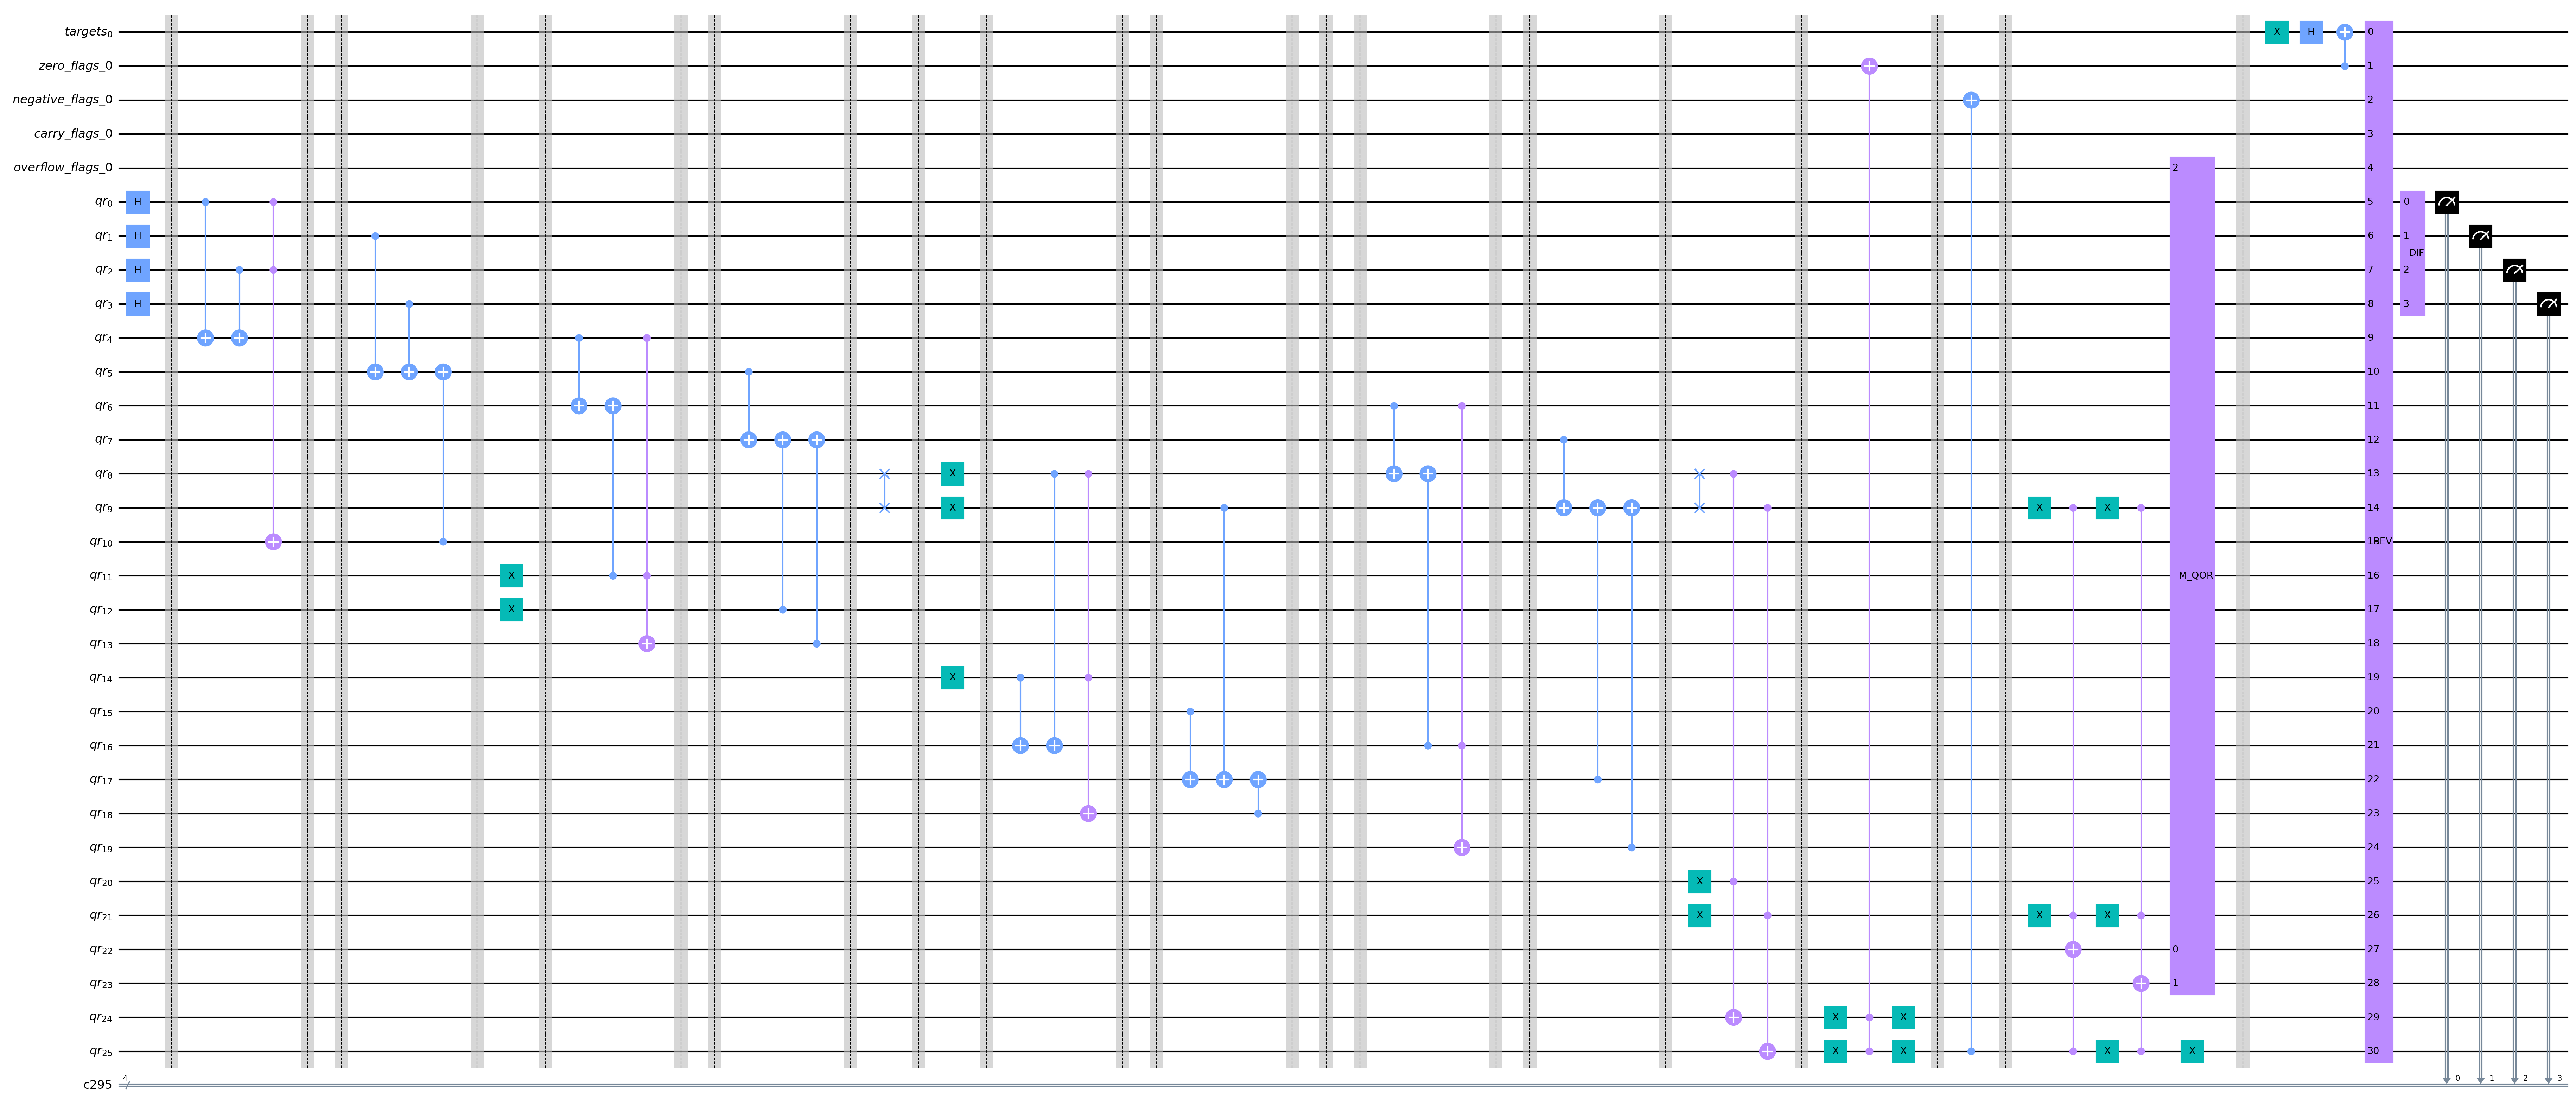
\includegraphics[width=9cm]{Figures/3-Partition_circuit.png}
    \caption{Using Grover's Algorithm to Solve the 3-Partition Problem}
    \label{fig:3-Partition}
\end{figure}

\section{Conclusion}

In this paper, we have proposed a novel approach to solving the 3-Partition problem using Grover's Algorithm. We have presented a detailed description of our method, including the construction of a quantum oracle for the 3-Partition problem and the use of Grover's Algorithm to efficiently search for a solution. Our approach leverages the power of quantum computing to potentially achieve significant improvements in efficiency compared to classical algorithms.

The quadratic speedup of Grover's Algorithm over classical search algorithms makes it a promising candidate for addressing various combinatorial search problems, including the 3-Partition problem. As quantum computing technology continues to advance, our proposed method could have far-reaching implications for the broader field of combinatorial optimization and the study of NP-complete problems.

Future research directions may include the exploration of alternative quantum algorithms for solving the 3-Partition problem and other NP-complete problems. Additionally, the implementation of our proposed method on actual quantum hardware would be an important step towards demonstrating its practical relevance. Furthermore, the development of efficient techniques for constructing quantum oracles for other combinatorial optimization problems would contribute to the broader applicability of quantum computing in solving complex computational challenges.

In conclusion, our work presents a promising approach to solving the 3-Partition problem using Grover's Algorithm, with potential implications for the broader field of quantum computing and combinatorial optimization. As quantum computing technology matures, the efficient solution of NP-complete problems like the 3-Partition problem may become increasingly feasible, opening new frontiers in both theoretical and applied research.

